\chapter{Sprint 2 : données de paie, schémas XSD et génération du fichier SEPA}
\label{ch:sprint2}
\startcontents[chapters]
\chapterplan

\section{Introduction}

Le deuxième sprint construit le c\oe ur fonctionnel de la plateforme : transformer des fiches de paie en un fichier \texttt{pain.001} conforme à un schéma choisi. Il couvre la saisie et l'approbation des fiches, la gestion des schémas XSD, la génération du message et sa validation, avec des messages d'erreur compréhensibles par un utilisateur non spécialiste. Planifié sur quatre semaines (tableau~\ref{tab:sprints}), il livre le noyau technique sur lequel s'appuie, au sprint suivant, le parcours complet de virement de masse.

\section{Backlog du sprint}

Le sprint reprend les récits US7 à US11 du backlog produit (tableau~\ref{tab:backlog}). Le tableau~\ref{tab:backlog-s2} précise les tâches associées.

\begin{table}[H]
\centering
\footnotesize
\renewcommand{\arraystretch}{1.1}
\tablestyle
\begin{tabularx}{\textwidth}{|>{\centering\arraybackslash}p{0.9cm}|>{\raggedright\arraybackslash}p{5.2cm}|Y|}
\hline
\rowcolor{appMarine}\entete{N\textsuperscript{o}} & \entete{Récit utilisateur} & \entete{Principales tâches} \\
\hline
US7 & Saisir des fiches de paie pour mes sociétés et les supprimer & Formulaire de saisie avec choix de la société ; contrôle d'accès par société ; suppression avec confirmation \\
\hline
US8 & Approuver les fiches de paie & Approbation par le Manager ; vérification des données avant approbation ; traçabilité \\
\hline
US9 & Importer et gérer les schémas XSD & Import, mise à jour et suppression de schémas ; droits réservés à l'administrateur et au Manager \\
\hline
US10 & Générer un fichier \texttt{pain.001} selon le schéma choisi & Lecture de la version et de la structure du schéma ; construction du message ; adaptation aux versions \\
\hline
US11 & Valider le fichier contre le XSD et en prévisualiser le contenu & Validation avec collecte de toutes les erreurs ; messages en clair ; aperçu du XML ; enregistrement dans l'historique \\
\hline
\end{tabularx}
\caption{Backlog du sprint 2}
\label{tab:backlog-s2}
\end{table}

\section{Conception}

\subsection{Diagramme de cas d'utilisation}

La figure~\ref{fig:uc-s2} présente les cas d'utilisation du sprint. L'Expert RH saisit et supprime les fiches, puis génère, prévisualise et télécharge le fichier. Le Manager approuve les fiches, tandis que la gestion des schémas XSD est partagée entre le Manager et l'administrateur. La génération du fichier inclut deux étapes systématiques : l'analyse du schéma choisi et la validation du résultat contre ce schéma.

\begin{figure}[H]
\centering
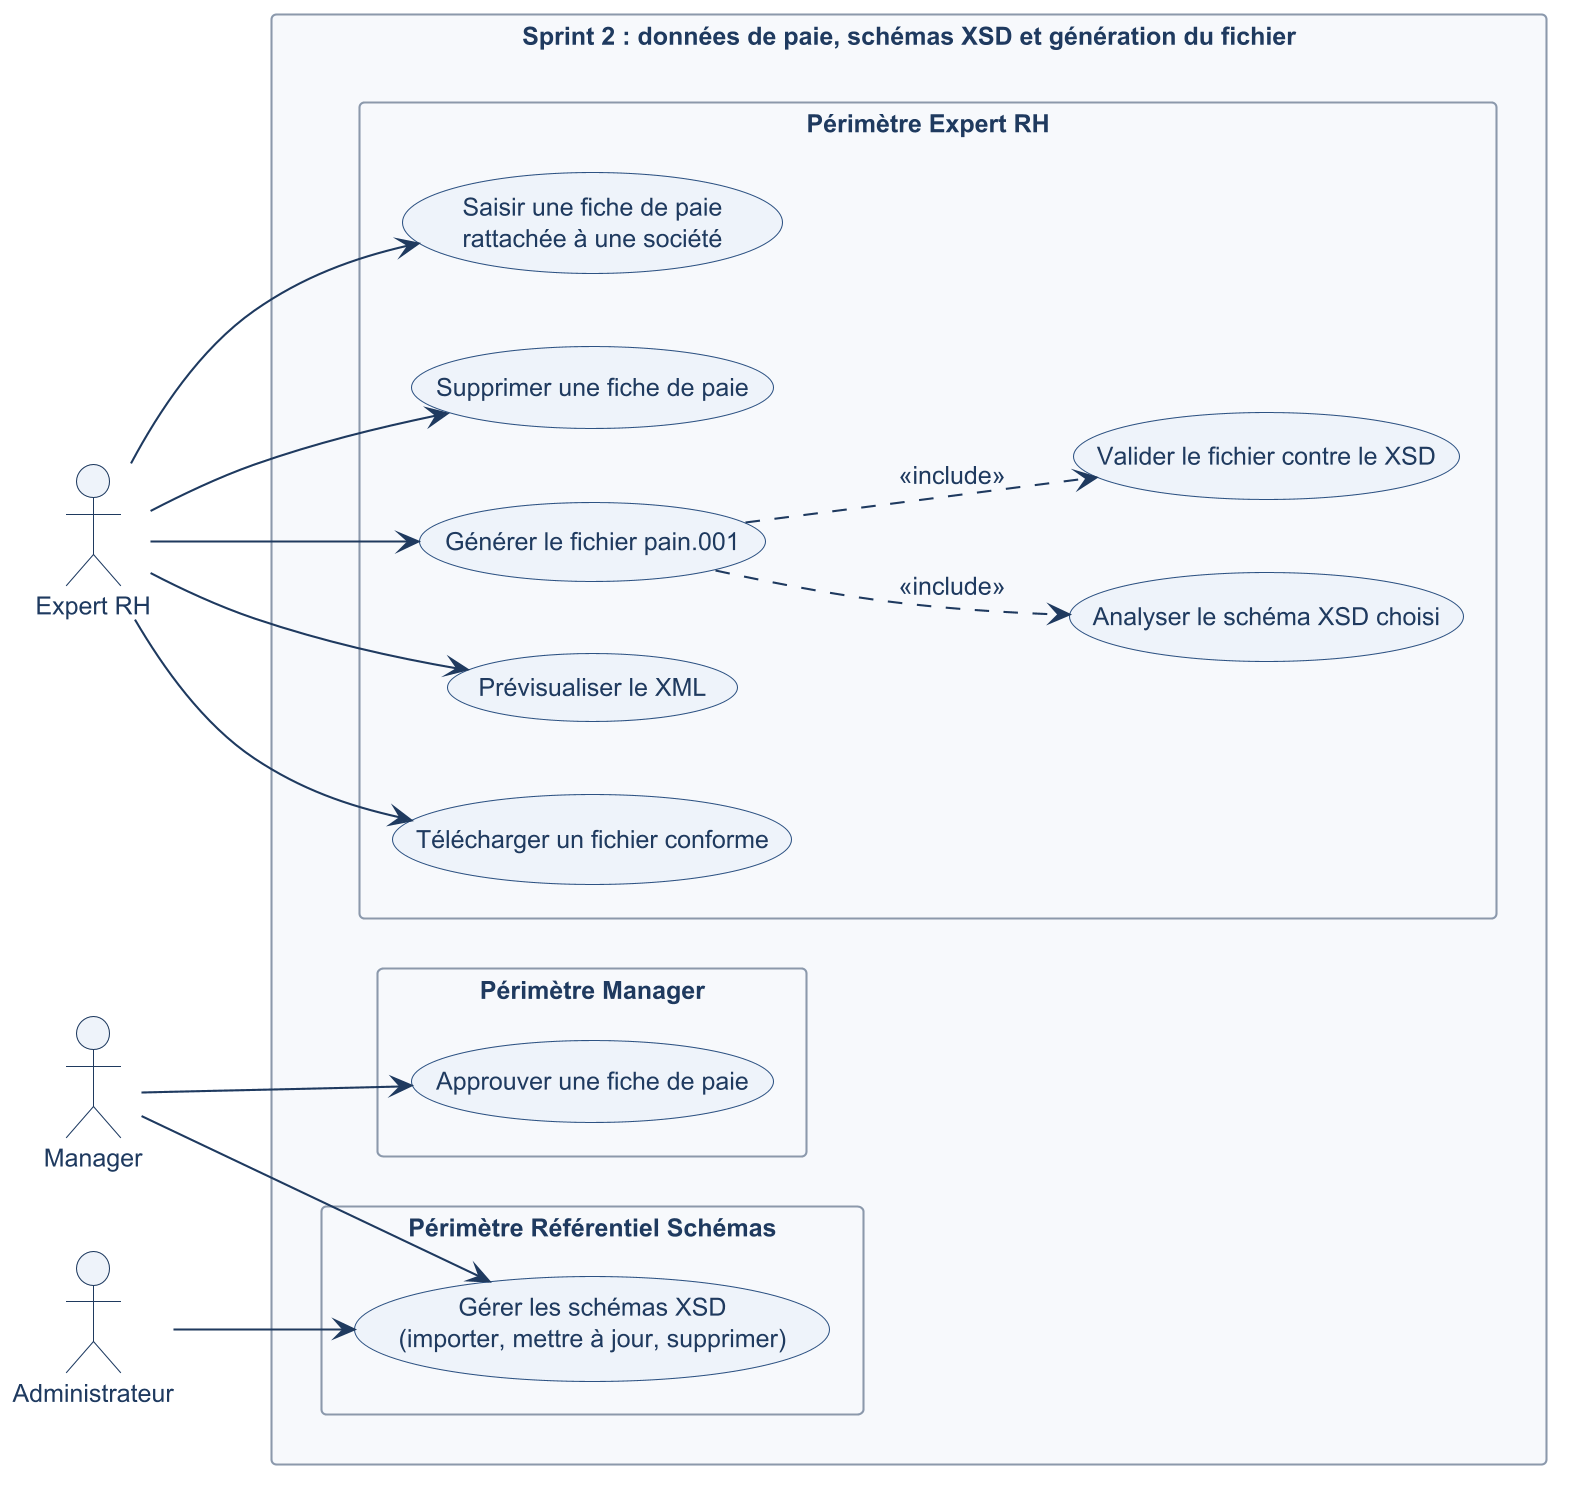
\includegraphics[width=\textwidth,height=0.36\textheight,keepaspectratio]{fig5_1_cas_utilisation_sprint2}
\caption{Cas d'utilisation du sprint 2}
\label{fig:uc-s2}
\end{figure}

\subsection{Cycle de vie d'une fiche de paie}

Une fiche de paie correspond à un virement individuel destiné à un salarié. Elle est saisie à l'état \textbf{brouillon}, puis approuvée par le Manager. Seules les fiches approuvées peuvent entrer dans un fichier SEPA. Cette séparation entre la personne qui saisit et celle qui approuve répète, à l'échelle de la fiche, le principe des quatre yeux présenté au chapitre~\ref{ch:besoins}. La figure~\ref{fig:etats-fiche} résume ce cycle de vie.

\begin{figure}[H]
\centering
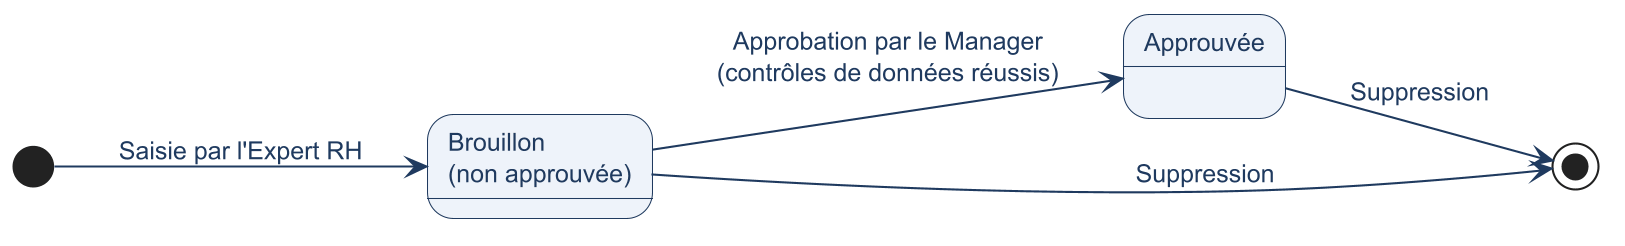
\includegraphics[width=\textwidth]{fig5_2_etats_fiche}
\caption{Cycle de vie d'une fiche de paie}
\label{fig:etats-fiche}
\end{figure}

\subsection{Chaîne de génération et de validation}

La génération du fichier suit une chaîne en plusieurs étapes, illustrée par la figure~\ref{fig:generation}. Le schéma choisi n'est pas seulement un outil de contrôle appliqué à la fin : il guide aussi la construction du message, dont certains éléments dépendent de la version. La plateforme analyse donc d'abord le schéma, construit le document en conséquence, puis le valide et présente le résultat. En cas de non-conformité, le fichier ne peut être ni téléchargé ni soumis.

\begin{figure}[H]
\centering
\begin{tikzpicture}[
  etape/.style={draw=appMarine, fill=appClair, rounded corners=3pt, align=center, text width=4.4cm, minimum height=1.25cm, font=\small, execute at begin node={\hyphenpenalty=10000\relax}},
  refus/.style={draw=acteurSysteme, fill=orange!8, dashed, rounded corners=3pt, align=center, text width=4.4cm, minimum height=1.0cm, font=\small, execute at begin node={\hyphenpenalty=10000\relax}},
  choix/.style={draw=acteurSysteme, fill=orange!8, diamond, aspect=2.6, inner sep=1pt, align=center, font=\small},
  fleche/.style={-{Stealth[length=2.4mm]}, appMarine, thick}]
\node[etape] (a) {1. Sélection des fiches\\approuvées et choix du schéma};
\node[etape, right=0.7cm of a] (b) {2. Analyse du schéma\\(version, structure)};
\node[etape, right=0.7cm of b] (c) {3. Construction du\\document XML};
\node[refus, above=0.9cm of b] (x) {Refus avec\\message explicatif};
\node[etape, below=0.9cm of c] (d) {4. Validation contre le XSD\\(toutes les erreurs)};
\node[etape, below=0.9cm of b] (e) {5. Messages d'erreur\\en clair (ligne, balise)};
\node[choix, below=0.9cm of a] (f) {Fichier conforme ?};
\node[etape, below=1.0cm of f] (g) {Enregistrement (statut\\Brouillon), contenu figé ;\\téléchargement possible};
\node[refus, right=0.7cm of g] (h) {Erreurs présentées ;\\téléchargement et soumission\\refusés};
\draw[fleche] (a) -- (b);
\draw[fleche] (b) -- (c);
\draw[fleche, acteurSysteme] (b) -- (x) node[midway, right, font=\scriptsize, text=black] {schéma incompatible};
\draw[fleche] (c) -- (d);
\draw[fleche] (d) -- (e);
\draw[fleche] (e) -- (f);
\draw[fleche] (f.south) -- (g.north) node[midway, right, font=\scriptsize] {oui};
\draw[fleche] (f.south) -- ++(0,-0.5) -| (h.north) node[pos=0.2, above, font=\scriptsize] {non};
\end{tikzpicture}
\caption{Chaîne de génération et de validation d'un fichier \texttt{pain.001}}
\label{fig:generation}
\end{figure}

\subsection{Fiches de paie et approbation}

Une fiche de paie comporte l'identifiant du salarié, le nom du bénéficiaire, son IBAN, un BIC facultatif, le montant, la devise (l'euro par défaut), un libellé et le code de la société débitrice. L'Expert RH la saisit pour l'une des sociétés qui lui sont affectées : le serveur refuse la saisie si la société est inconnue, inactive ou non affectée à l'utilisateur, et la liste proposée dans le formulaire est déjà limitée à ses sociétés. Le montant doit être strictement positif. Dans les listes, l'IBAN est masqué et la création comme la suppression d'une fiche sont tracées dans le journal d'audit.

L'approbation est réservée au Manager. Avant de la prononcer, le serveur vérifie les données de la fiche : IBAN valide (format et clé de contrôle), BIC bien formé s'il est renseigné et montant positif. Si l'une de ces vérifications échoue, la fiche reste en brouillon et le message indique ce qu'il faut corriger. Ces règles, communes à plusieurs étapes de la plateforme, sont détaillées au chapitre~\ref{ch:sprint3}. Dans le cadre du projet, les fiches proviennent de cette saisie unitaire ou de jeux de données synthétiques chargés en base pour la démonstration et l'évaluation ; un import automatique depuis le SIRH n'est pas réalisé.

\subsection{Gestion des schémas XSD}

Un schéma XSD est importé sous forme de fichier. Il est conservé avec son nom, son contenu, le nom de l'utilisateur qui l'a importé et sa date d'import. Importer à nouveau un fichier de même nom crée une nouvelle version, et la mise à jour d'un schéma existant en incrémente également le numéro de version. La suppression est possible. L'import, la mise à jour et la suppression sont réservés à l'administrateur et au Manager, et chacune de ces opérations est enregistrée dans le journal d'audit. Tous les utilisateurs authentifiés peuvent en revanche consulter la liste des schémas disponibles.

L'import n'impose pas qu'un fichier soit un schéma \texttt{pain.001}. La compatibilité est vérifiée au moment de l'utilisation : un schéma qui ne décrit pas l'élément \texttt{CstmrCdtTrfInitn} est signalé comme incompatible et ne peut pas servir à générer un fichier. Ce choix permet de conserver d'autres schémas, par exemple d'autres versions, sans bloquer leur import.

\subsection{Analyse dynamique du schéma}

Pour construire un message cohérent avec le schéma choisi, la plateforme en lit la structure. Elle extrait d'abord la version et l'espace de noms, puis parcourt l'arbre des éléments à partir de \texttt{CstmrCdtTrfInitn}. Pour chaque élément, elle relève s'il est obligatoire, s'il peut se répéter, son type et ses contraintes : longueur maximale ou minimale, format, nombre de chiffres, liste de valeurs autorisées. Le test sur le schéma officiel \texttt{pain.001.001.03} confirme par exemple que l'identifiant du message est limité à 35 caractères et le nom d'une partie à 140.

Cette lecture est protégée de deux manières. Elle est bornée en profondeur et en nombre d'éléments, et elle détecte les définitions circulaires, afin qu'un schéma volumineux ou mal conçu ne bloque pas le serveur. Elle interdit aussi les déclarations de type de document et l'accès aux ressources externes, ce qui écarte les attaques par entités externes déjà évoquées pour les besoins non fonctionnels.

\subsection{Génération du fichier \texttt{pain.001}}

Le document est construit avec l'interface standard de manipulation d'arbres XML, puis sérialisé avec indentation. Il comporte un en-tête de groupe, un lot de paiement unique pour la société débitrice, puis une instruction par fiche. Le nombre de virements et la somme de contrôle sont calculés à partir des fiches sélectionnées. Le lot porte le niveau de service \texttt{SEPA} et la catégorie \texttt{SALA}, qui qualifie un virement de salaire. Les coordonnées de la société débitrice proviennent de sa fiche, présentée au chapitre~\ref{ch:sprint1}.

Plusieurs versions du message coexistent. Pour les versions \texttt{pain.001.001.09} à \texttt{.11}, le code de la banque est porté par l'élément \texttt{BICFI} et la date d'exécution est encapsulée dans un élément \texttt{Dt} ; pour la version \texttt{.03}, ils utilisent respectivement \texttt{BIC} et une date simple. La version est lue dans le schéma choisi et le générateur adapte le message en conséquence.

Les valeurs saisies ne respectent pas toujours les contraintes du standard. Le générateur les prépare donc selon les règles du tableau~\ref{tab:preparation-valeurs}. Lorsqu'un champ facultatif est vide, comme le nom d'une partie ou le BIC, et que le schéma l'autorise, la balise est omise et un avertissement non bloquant est produit. Un champ obligatoire vide reste en revanche une erreur de validation.

\begin{table}[H]
\centering
\small
\renewcommand{\arraystretch}{1.2}
\tablestyle
\begin{tabularx}{\textwidth}{|>{\raggedright\arraybackslash}p{4.2cm}|Y|}
\hline
\rowcolor{appMarine}\entete{Donnée} & \entete{Préparation appliquée} \\
\hline
Noms et libellés & Suppression des accents, remplacement des caractères hors du jeu autorisé, puis troncature : 70 caractères pour un nom, 140 pour le libellé \\
\hline
Identifiants du message et des virements & Identifiant unique composé de la date et d'une partie aléatoire ; référence de bout en bout construite à partir du matricule et de la période ; troncature à 35 caractères \\
\hline
Montants & Deux décimales, avec le point comme séparateur \\
\hline
IBAN et BIC & Suppression des espaces et passage en majuscules \\
\hline
Date d'exécution & Valeur demandée, ou à défaut le jour courant augmenté de deux jours \\
\hline
Libellé du virement & \og Salaire\fg{} suivi du mois, de l'année et du matricule \\
\hline
\end{tabularx}
\caption{Préparation des valeurs lors de la génération}
\label{tab:preparation-valeurs}
\end{table}

\subsection{Validation XSD et messages d'erreur}

Le document généré est validé contre le schéma choisi. Par défaut, un validateur s'arrête à la première erreur et produit des messages techniques en anglais, difficiles à exploiter. SEPAPaie collecte donc \textbf{toutes} les erreurs en une seule passe. Pour chacune, elle conserve la ligne, la colonne et la balise concernée, puis la traduit en un message en français qui indique la correction à apporter. Plusieurs diagnostics situés au même endroit sont regroupés, et un message particulier distingue l'IBAN du débiteur de celui d'un bénéficiaire.

Le tableau~\ref{tab:erreurs-xsd} donne des exemples de messages obtenus. L'utilisateur n'a ainsi pas besoin de connaître le vocabulaire du standard pour comprendre ce qu'il doit corriger.

\begin{table}[H]
\centering
\small
\renewcommand{\arraystretch}{1.2}
\tablestyle
\begin{tabularx}{\textwidth}{|>{\raggedright\arraybackslash}p{3.6cm}|Y|}
\hline
\rowcolor{appMarine}\entete{Situation} & \entete{Message restitué à l'utilisateur (reformulé)} \\
\hline
Valeur trop longue & Le nom est trop long ; raccourcissez-le au nombre de caractères maximal du schéma \\
\hline
IBAN au format incorrect & L'IBAN du compte concerné est incorrect ; il doit comporter deux lettres de pays, deux chiffres de contrôle, puis le numéro de compte, sans espace \\
\hline
Date invalide & La date d'exécution est invalide ; utilisez une date réelle au format année-mois-jour \\
\hline
Montant invalide & Le montant est invalide ; utilisez un nombre avec un point décimal, sans devise ni séparateur de milliers \\
\hline
Balise manquante ou mal placée & Une balise est manquante, inattendue ou placée dans le mauvais ordre ; le message précise la balise attendue \\
\hline
\end{tabularx}
\caption{Exemples de messages d'erreur de validation XSD}
\label{tab:erreurs-xsd}
\end{table}

\subsection{Aperçu, enregistrement et téléchargement}

L'Expert RH peut d'abord prévisualiser le fichier sans l'enregistrer. L'aperçu présente le XML généré, le résultat de la validation et les erreurs éventuelles. Lorsque le fichier est conforme, il peut être enregistré dans l'historique. L'enregistrement conserve le contenu XML, le schéma utilisé et sa version, la société et la période, les matricules et les identifiants des fiches incluses, le nombre de virements, la somme de contrôle, les coordonnées du débiteur, le résultat de la validation, l'auteur et la date. Le fichier reçoit alors le statut \og Brouillon\fg{}.

Le contenu XML n'est jamais modifié après l'enregistrement : un téléchargement ultérieur restitue exactement le même document, ce qui permet de le rapprocher du fichier remis à la banque. Un fichier non conforme ne peut pas être téléchargé. Le téléchargement d'un fichier qui n'a pas encore été validé par le Manager donne un nom préfixé par \og NON\_VALIDE\fg{}, afin d'éviter qu'il soit confondu avec un fichier validé. Chaque téléchargement est tracé. L'historique peut être filtré par société, période, conformité et statut, et un Expert RH n'y voit que les fichiers de ses sociétés. Le parcours complet, qui enchaîne contrôles métier, analyse par l'IA et validation XSD en conservant aussi les résultats non conformes pour consultation, est présenté au chapitre~\ref{ch:sprint3}.

\subsection{Interfaces réalisées}

La figure~\ref{fig:ecran-saisie} montre la saisie d'une fiche par un Expert RH : la société est choisie parmi celles qui lui sont affectées. Le tableau indique la société sous le matricule, le statut de la fiche et, dans les colonnes de droite, les informations du module d'IA présenté au chapitre~\ref{ch:sprint4}.

\begin{figure}[H]
\centering
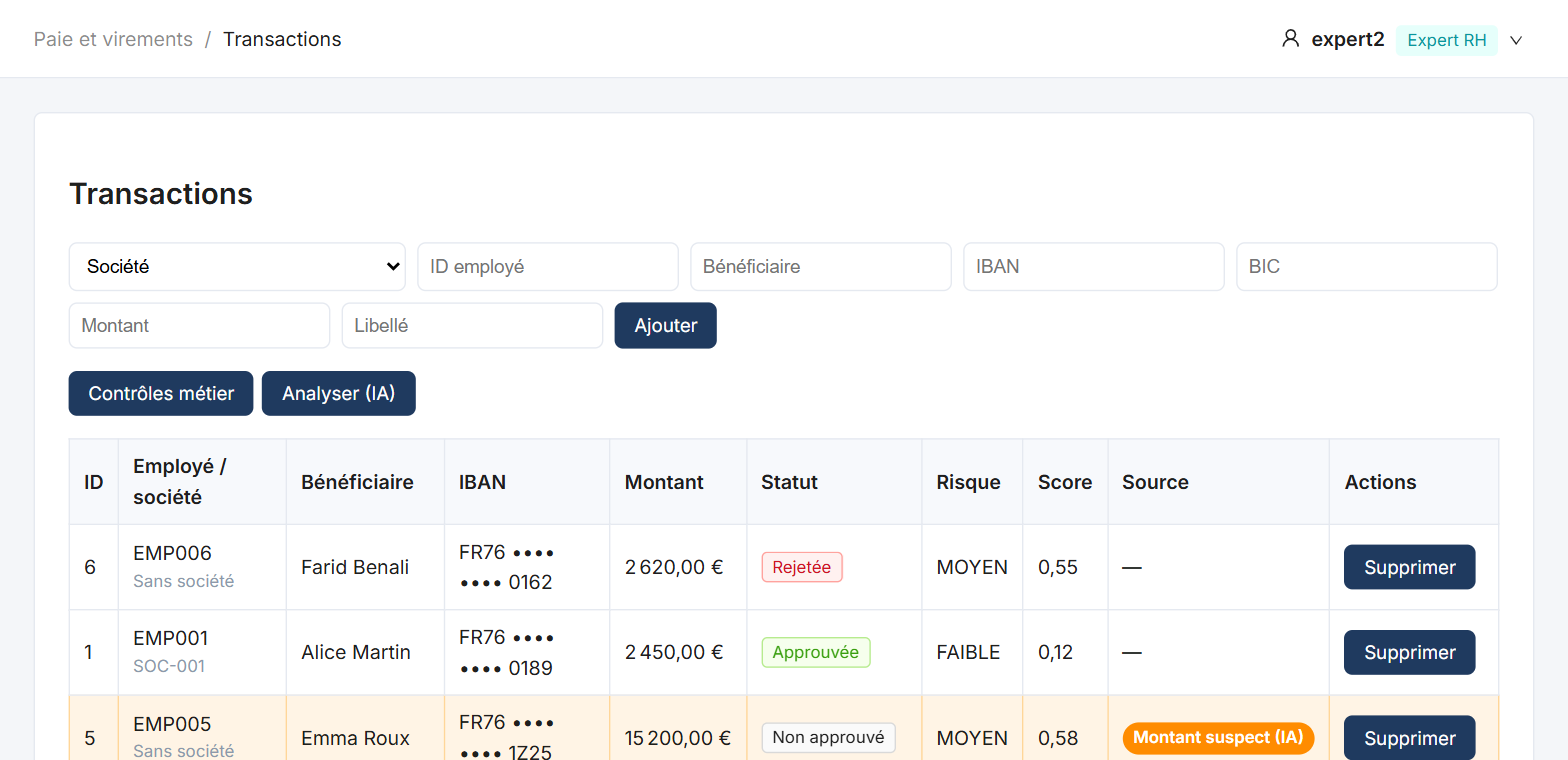
\includegraphics[width=0.95\textwidth]{fig5_saisie_fiche}
\caption{Saisie d'une fiche de paie (profil Expert RH)}
\label{fig:ecran-saisie}
\end{figure}

Les figures~\ref{fig:ecran-xml} et~\ref{fig:ecran-validation} montrent le résultat d'un fichier généré. L'onglet XML présente le document avec une coloration syntaxique ; les lignes en erreur ou en avertissement y sont mises en évidence. L'onglet de validation indique la conformité au schéma et liste, le cas échéant, les erreurs avec leur ligne et leur balise.

\begin{figure}[H]
\centering
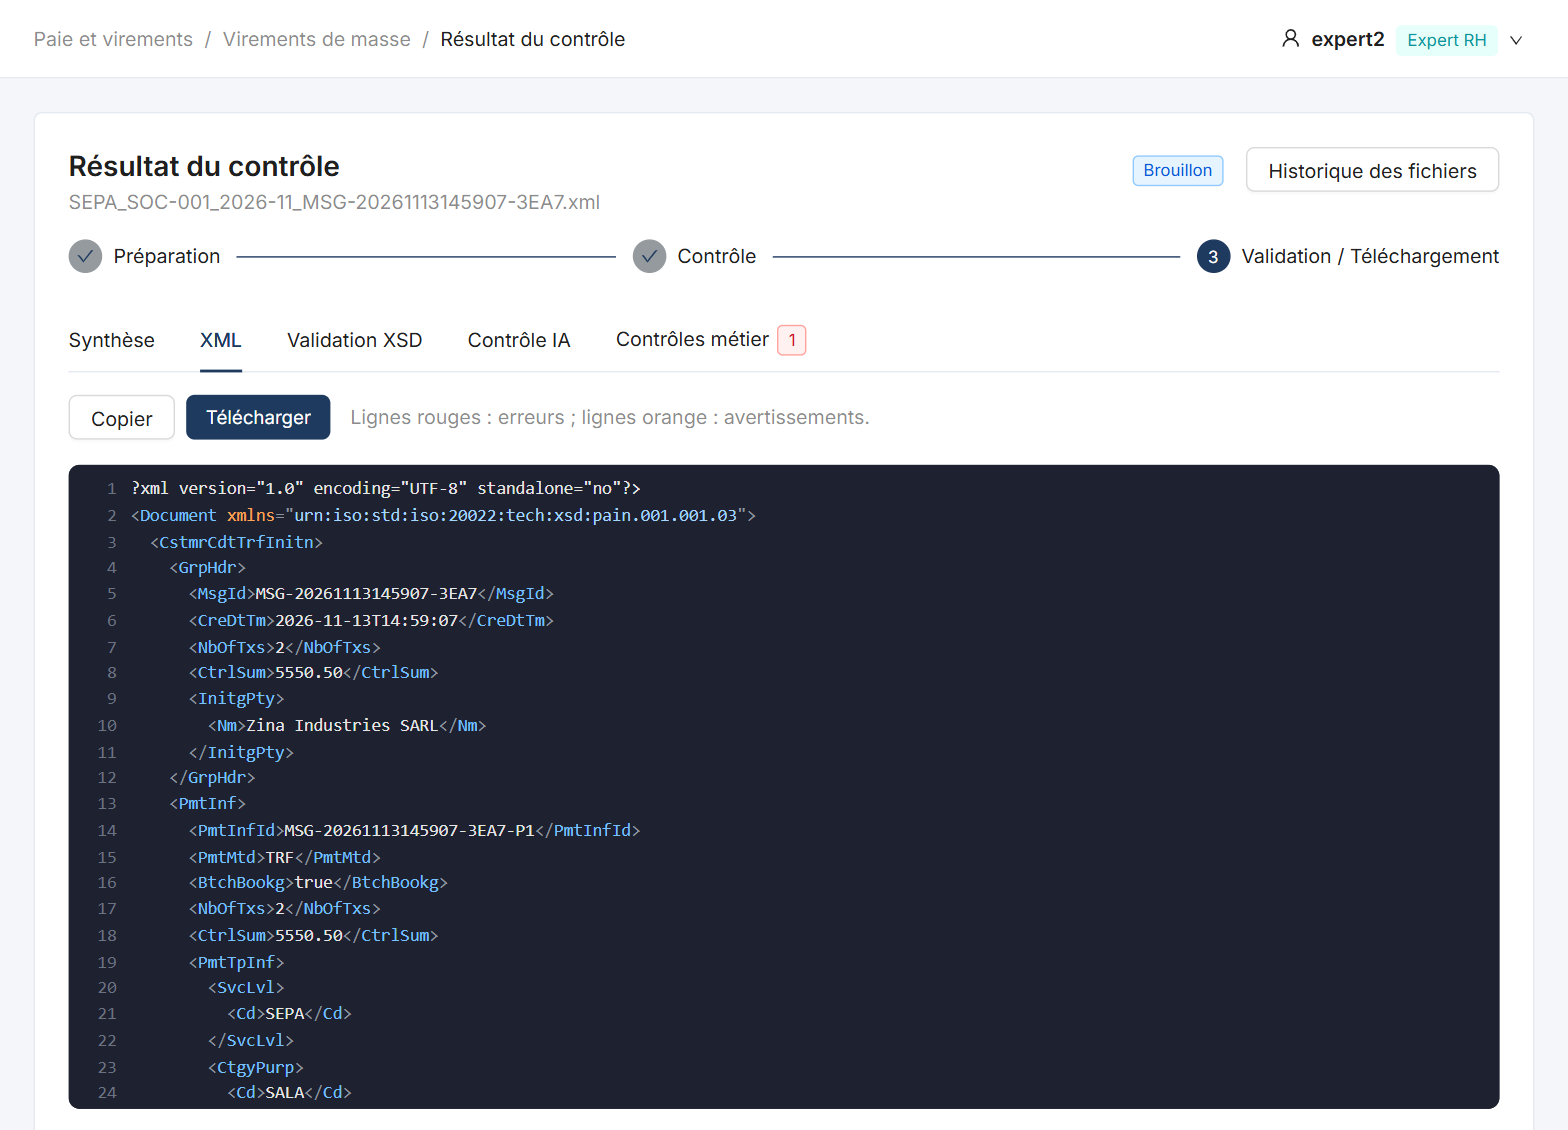
\includegraphics[width=0.95\textwidth]{fig5_xml}
\caption{Aperçu du fichier XML généré}
\label{fig:ecran-xml}
\end{figure}

\begin{figure}[H]
\centering
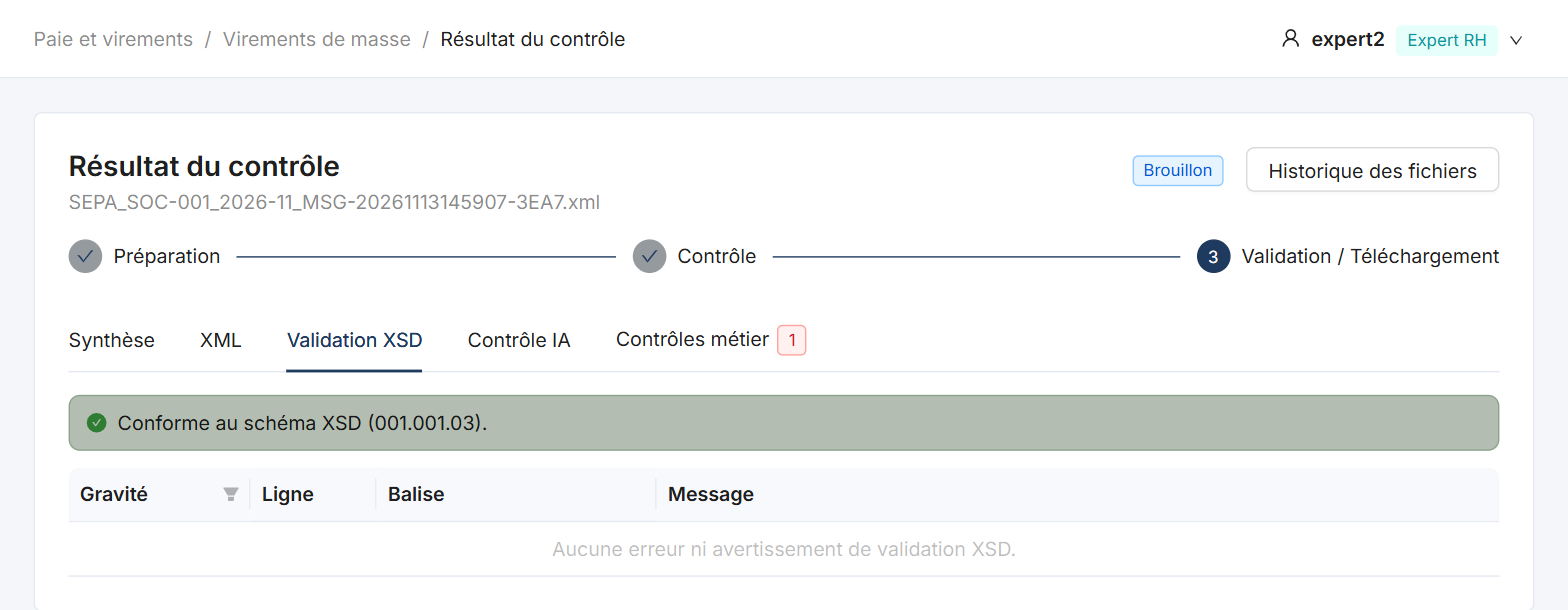
\includegraphics[width=0.95\textwidth]{fig5_validation_xsd}
\caption{Résultat de la validation XSD}
\label{fig:ecran-validation}
\end{figure}

\section{Conclusion}

Le sprint 2 a livré le noyau technique de la plateforme : fiches de paie rattachées à une société et approuvées avant tout usage, schémas XSD gérés par les profils autorisés, fichier \texttt{pain.001} construit selon la version du schéma, et validation qui restitue toutes les erreurs en langage clair. Le chapitre suivant présente le sprint 3, qui enchaîne ces briques dans un parcours de virement de masse avec contrôles métier et circuit de validation.

